%
% ================================================================
% 

\begin{frame}{\textbf{OSP} $\mid$ Definition $\mid$ One machine scheduling problem}

The general one machine scheduling problem considered here is defined as:

$$ \hspace{30mm} 1\mid r_i \mid (f_1,f_2)  \hspace{30mm} \mbox{(2-OSP)}$$
\medskip 

and the specific OSP  currently considered is:

$$1\mid . \mid (\Sigma C_i,T_{max}) \hspace{12mm}$$

\end{frame}

%
% ================================================================
% 
\begin{frame}{OSP $\mid$ Definition $\mid$ Inputs}

Valid for 2-OSP.
\bigskip
              \begin{itemize}
                \item \texttt{n} (integer): \\ number $n$ of jobs, $i=1\dots n$   
                                           \medskip
                \item \texttt{r} (vector of $n$  integers): \\   $r_{i}$,  the release date for job $i$                
                                           \medskip    
                \item \texttt{p} (vector of $n$  integers): \\   $p_{i}$, the processing time for job $i$         
                                           \medskip    
                \item \texttt{d} (vector of $n$  integers): \\  $d_{i}$, the due date for job $i$     
                                           \medskip
                \item \texttt{w} (vector of $n$  integers): \\  $w_{i}$, the weight associated to job $i$                              
              \end{itemize}
\end{frame}

%
% ================================================================
% 
\begin{frame}[fragile=singleslide]{OSP $\mid$ Data $\mid$ Example (console)}

{\small
\begin{verbatim}
n = 4
p = [  2   4   3   1 ]
d = [  1   2   4   6 ]
r = [  0   0   0   0 ]
w = [  1   1   1   1 ]
\end{verbatim}
}

\end{frame}

%
% ================================================================
% 
\begin{frame}[fragile=singleslide]{OSP $\mid$ Data $\mid$ Example (text file)}

\begin{columns}
\begin{column}{0.3\textwidth}
{\small
\begin{verbatim}
4
2   4   3   1 
1   2   4   6 
0   0   0   0 
1   1   1   1 
\end{verbatim}
\vspace{1mm}
}
\end{column}
\begin{column}{0.3\textwidth}
\vspace{-2mm}
%\begin{center}
\hspace{-5mm}
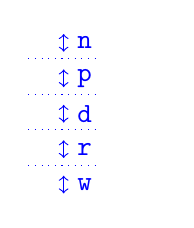
\begin{tikzpicture}[scale=0.45]%[auto]

\draw  [<->, color=blue](0,1.2) -- (0,1.7);
\draw  [<->, color=blue](0,2.2) -- (0,2.7);
\draw  [<->, color=blue](0,3.2) -- (0,3.7);
\draw  [<->, color=blue](0,4.2) -- (0,4.7);
\draw  [<->, color=blue](0,5.2) -- (0,5.7);

\node [text width=1cm,align=left, color=blue] at (1.5,5.45) {{\texttt{n}}};
\node [text width=1cm,align=left, color=blue] at (1.5,4.45) {{\texttt{p}}};
\node [text width=1cm,align=left, color=blue] at (1.5,3.45) {{\texttt{d}}};
\node [text width=1cm,align=left, color=blue] at (1.5,2.45) {{\texttt{r}}};
\node [text width=1cm,align=left, color=blue] at (1.5,1.45) {{\texttt{w}}};

\draw  [-, dotted, color=blue](-1,5) -- (1,5);
\draw  [-, dotted, color=blue](-1,4) -- (1,4);
\draw  [-, dotted, color=blue](-1,3) -- (1,3);
\draw  [-, dotted, color=blue](-1,2) -- (1,2);
\end{tikzpicture}
\vfill
\end{column}
\begin{column}{0.15\textwidth}

\end{column}
\end{columns}

\vspace{10mm}
\begin{itemize}
\item  \blue{load2OSP}\\
          Load an instance of a 2-OSP from the file \texttt{fname}    \\
           \texttt{id = \texttt{{load2OSP}( fname ) }} 
           \medskip
\end{itemize}

\end{frame}

%
% ================================================================
% 
\begin{frame}{OSP $\mid$ Resolution $\mid$ API}

\begin{itemize}
\item  \blue{set2OSP}\\
          Create a new instance of a 2-OSP and set up all required values    \\
           \texttt{id = \texttt{{set2OSP}( n , P, D, R, W ) }} 
           \medskip
\item  \blue{OSP\_vanwassenhove1980} \\
          Set up the solver to use for the 2-OSP\\
          \texttt{solver = OSP\_vanwassenhove1980( ) }
          \medskip
\item  \blue{vSolve}\\
          Solve an instance of a 2OSP with the mentioned solver and return the results \\
          \texttt{status = vSolve( id , solver ) }
          \medskip
%\item  \red{get2OSP}\\
%          Retrieve the results  \\
%          \texttt{results = \red{get2OSP}( id ) }         
\end{itemize}

\end{frame}

%
% ================================================================
% 
\begin{frame}{OSP $\mid$ Resolution $\mid$ Outputs (specification)}

Valid for 2-OSP.
\bigskip

vSolve returns:
\medskip
                           \begin{itemize}
                            %  \item $CPUt$: \\ the time consumed
%                              \item $nYn$: \\ the number of non-dominated points
                              \item z1: vector of ($1, \dots, \mid Y_N \mid $) of integers
                              \item z2: vector of ($1,\dots, \mid Y_N \mid $) of integers
                              \item $\sigma$: matrix of ($1,\dots, \mid Y_N \mid $ ; $\sigma_1, \dots, \sigma_n$) of integers
                                                                                         
%                              $$ z_1, z_2, \sigma_1, \dots, \sigma_n$$
                              where
                               \begin{itemize}
%                                     \item $z_k, \ k=1,\dots,p$ of integers:  performances 
                                     \item $\sigma_i$:  a permutation coding ($\sigma_i=j  \Leftrightarrow \mbox{ job } j \mbox{ in position } i$)
                                \end{itemize}
                           \end{itemize}               

\end{frame}

%Non-dominated parts of the 2-LAP is defined by a set of points:
%\medskip
%                           \begin{itemize}
%                             % \item $CPUt$: \\ the time consumed
%                              \item $nYn$: \\ the number of non-dominated points
%                              \item $Yn$: \\the list of points,  each point is defined by 
%                              $$ z_1, z_2, \sigma_1, \dots, \sigma_n$$
%                              where
%                               \begin{itemize}
%                                     \item $z_k, \ k=1,\dots,p$ of integers:  performances 
%                                     \item $\sigma_i, \ i=1,\dots,n$ of integers:  permutation coding ($\sigma_i=j  \Leftrightarrow \mbox{ job } j \mbox{ in position } i$)
%                                \end{itemize}
%                           \end{itemize}               



%
% ================================================================
% 
%\begin{frame}{OSP $\mid$ Resolution $\mid$ Outputs (text file)}
%\red{a ecrire}
%\end{frame}
